\documentclass{article}

\usepackage[utf8x]{inputenc}
\usepackage[spanish]{babel}
\usepackage[margin=2.7cm]{geometry}
\usepackage{amsmath}
\usepackage{amssymb}
\usepackage{graphicx}
\usepackage{algorithm}
\usepackage{algorithmic}

\usepackage{ stmaryrd }

\usepackage{ upgreek }

\usepackage{listings}

\linespread{1.0}

\usepackage{color}
\usepackage{listings}

\definecolor{javared}{rgb}{0.6,0,0} % for strings
\definecolor{javagreen}{rgb}{0.25,0.5,0.35} % comments
\definecolor{javapurple}{rgb}{0.5,0,0.35} % keywords
\definecolor{javadocblue}{rgb}{0.25,0.35,0.75} % javadoc
 
\lstset{language=Java,
basicstyle=\ttfamily,
keywordstyle=\color{javapurple}\bfseries,
stringstyle=\color{javared},
commentstyle=\color{javagreen},
morecomment=[s][\color{javadocblue}]{/**}{*/},
numbers=left,
numberstyle=\tiny\color{black},
stepnumber=1,
numbersep=10pt,
tabsize=4,
showspaces=false,
showstringspaces=false}

\title{ Computación Concurrente \\ \Large{Tarea 10}
\author{
  Diego Goméz Montesinos
  \and
  José Emiliano Cabrera Blancas
  }
\date{20 Mayo 2014}
}
\begin{document}
\maketitle
\begin{enumerate}
  
\item{
    \textsl{
      Hacer un resumen de a lo más una cuartilla de Don't Settle for
      Eventual Consistency.\\
    }
    
    El geo-replicamiento de datos provee copias de la misma
    información en multiples locaciones geograficamente distantes. En
    cada centro de datos, un grupo de servidores acepta peticiones
    HTTP y maneja esas peticiones escribiendo y leyendo informacion
    del sistema de almacenamiento.\\
    El geo-replicamiento provee de dos servicios Web clave: tolerancia
    a fallos y lantecia baja. La tolerancia a fallos se soluciana  a
    traves de la redudancia: si algún centro de datos falla, entonces
    otro puede tomar su lugar y proveer el servicio. Provee baja
    latencia a traves de la proximidad: los clientes hacen peticiones
    a servidores cercanos a ellos.\\
    Un sistema con consistencia fuerte siempre esta disponible para
    lecturas y escrituras, y cuando la red se
    particione el sistema puede continuar brindado
    servicio. Disponibilidad implica que el servicio siempre podra
    responderle a todos los usuarios, y la tolerancia al
    particionamiento de la red implica que el sistema pueda continuar
    cuando los centros de datos no se puedan conmunicar entre si.\\
    
    Consistencia Eventual\\
    
    La consistencia eventual es un termino usado para multiples
    significados. En este texto lo definiriemos de la siguiente forma:
    La escritura en un centro de datos eventualmente aparecera en los
    otros centros de datos y su todos los centros de datos reciben la
    misma información de escritura, entonces todos los datos tendran
    los mismo valores.\\
    Debemos fijarnos en que, aunque la consistencia eventual provee a
    los programadores una forma más fácil de hacer las cosas, esta no
    nos define un orden sobre las operaciones de escritura y
    lectura. Lo que significa que los distintos centro de datos solo
    reflejarian conjuntos distintos de operaciones.\\
    
    Consistencia Casual\\

    La concistencia casual nos asegura que las operaciones apareceran
    en el orden en el que el usuario espera que sucedan. Más
    precisamente, asegura que existira un orden parcial sobre las
    operaciones.\\
    Las tres condiciones que se cumples son:\\
    \begin{itemize}
      \item{\textbf{Hilo de ejecución}: Si a y b son dos operaciones que
          realiza un solo hijo de ejecución, entonces $a \rightarrow
          b$.}
      
      \item{\textbf{Lecturas-de}: Si a es una operaciones de escritura
        y b una de lectura que regresa el valor de a, entonces $a
        \rightarrow b$.}

      \item{\textbf{Transitividad}: Para las operaciones a, b y c, si
          $a \rightarrow b$ y $b \rightarrow c$, entonces $a
          \rightarrow b$}
    \end{itemize}
  }
  La consistencia casual deja felices a los usuarios, por que se
  asegura que las operaciones se aplicaran en todos los centro de
  datos en el orden en el que se hicieron.\\
  
  Aunque la consistencia casual soluciona un problema grave para
  sistemas como las redes sociales, no son una solución viable para
  sistemas donde la disponibilidad de los datos más actuales
  siempre sea requerido, como es el caso del sistema financiero.\\
  
\item{
    \textsl{
      En la figura se muestra una historia para tres procesos, cada
      línea corresponde a un proceso diferente.\\
      Los tres procesos trabajan sobre una pila s. Este objeto tiene
      dos métodos:
    }

    \begin{itemize}
    \item{\textsl{
          s.top(i) que indica que el elemento i esta en la casilla
          superior de la pila, pero no elimina al elemento i.
        }}
      
    \item{\textsl{
          s.push(i) que pone el elemento i en la casilla superior de la
          pila s.
    }
    
    \begin{centering}
      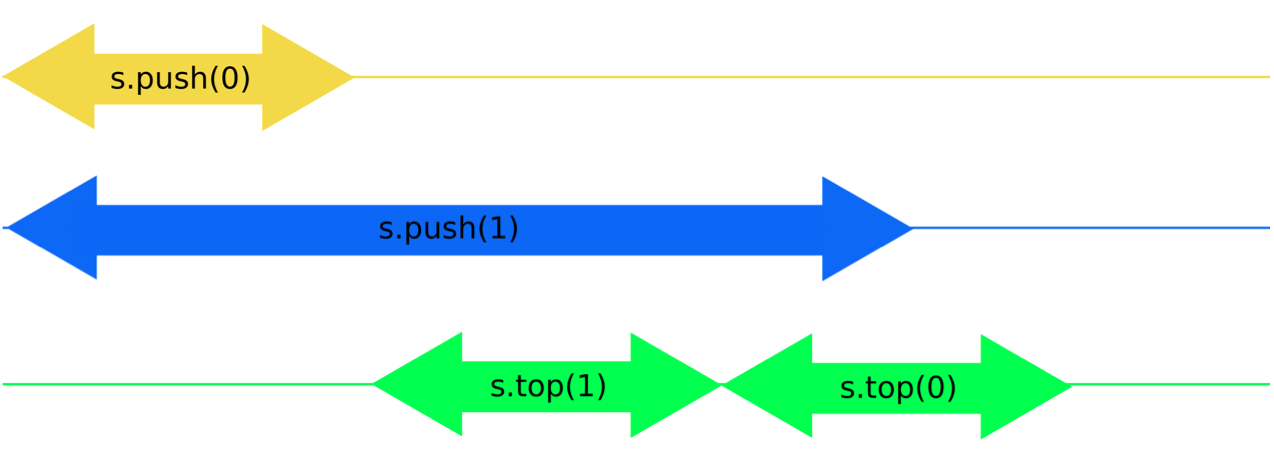
\includegraphics[scale=0.27]{figure1}
    \end{centering}
  }
\end{itemize}

\begin{enumerate}
  \item{\textsl{Indica si la historia es linearizable}}
  \\No es linearizable.
  \\\\Llamemosle al proceso amarillo A, al azul B y al verde C.
  \\Fijemonos en la primera llamada de C a s.top(): en esta llamada le
  es regresado $1$, lo cual significa que antes tuvo que tener efecto
  la llamada de B a s.push(1).
  \\Ahora, en la segunda llamada de C a s.top() le es regresado $0$.
  Recordemos que la operación s.top(i) solo regresa el elemento en la
  casilla superior, y no la elimina, además la segunda llamada de C está
  justo después de la primera llamada, por lo que esta tendría que haber
  regresado $1$ igual que la anterior.
  \\Esto es suponiendo que la llamada de B tuvo efecto después de la
  llamada de A.
  \\\\Si la llamada de A tiene efecto después de la llamada de B, entonces
  la primera llamada a s.top() de C tuvo que regresar 0, es decir, el valor
  de A pues fue el último.
  \\\\Por lo tanto no hay manera de acomodar los puntos de linearización.
  \item{\textsl{Indica si la historia es secuencialmente consistente}}
  \\Si es secuencialmente consistente.
  \\\\Considere el orden siguiente: B hace s.push(1), C lee con s.top(1),
  después A hace s.push(0) y por último C lee s.top(0).
\end{enumerate}

\item{\textsl{
      Considera el siguiente código.\\
      La clase \texttt{AtomicInteger} es un contenedor para un valor
      entero. Esta clase contiene el método \texttt{boolean
        CompareAndSet (int expect, int update)} que compara el valor
      actual del objeto con \texttt{expect}. Si los valores son
      iguales, entonces atómicamente se reemplaza el valor del objeto
      con el valor \texttt{update} y se devuelve \texttt{true}. Si los
      valores no son iguales, el objeto no cambia y se regrsa
      \texttt{false}. La clase también contiene el método \texttt{int
        get()} que regresa el valor actual del objeto.\\
      El código muestra la implementación de una cola FIFO. La cola
      guarda a los elementos en el arreglo \texttt{items}, el cual
      supondremos que tiene capacidad infinita; también contiene dos
      campos de la clase \texttt{AtomicInteger.head} que es el índice
      de la casilla del siguiente elemento a ser eliminado y
      \texttt{tail} que es el índice de la casilla en la que se
      guardará el siguiente elemento.
    }

    \renewcommand{\lstlistingname}{}
\begin{lstlisting}[frame=single]
class IQueue<T> f {
   AtomicInteger head = new AtomicInteger(0);
   AtomicInteger tail = new AtomicInteger(0);
   T[] items = (T[]) new Object[Integer.MAX VALUE];
   
   public void enq(T x){
      int slot;
      do {
         slot = tail.get();
      } while (! tail.compareAndSet(slot, slot + 1));
      items[slot] = x;
   }

   public T deq() throws EmptyException {
      T value;
      int slot;
      do {
         slot = head.get();
         value = items[slot];
         if (value == null) {
            throw new EmptyException();
         }
      } while (! head.compareAndSet(slot, slot + 1));
      return value;
   }
}
\end{lstlisting}
    \textsl{Da un ejemplo que muestre que esta implementación no es
      linearizable.}
    \\El problema que tiene esta implementación es que no sabemos si
    tenemos 3 procesos y dos son rápidos y uno lento, puede que el lento
    devuelva un valor anterior al que tenía que devolver. Como se muestra
    en la siguiente imagen:
    \\
    \begin{center}
      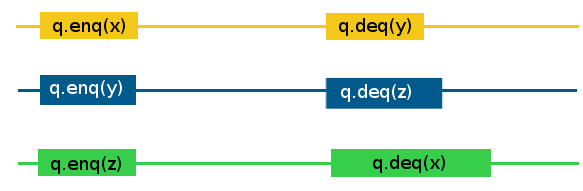
\includegraphics[scale=0.5]{figure2}
    \end{center} 
  }
}

\item{\textsl {
      En clase se vio como construir registros a partir de
      otros. Describir detalladamente el algoritmo que construye
      registros Multi-Writer Atomic a partir de los registros
      Multi-Reader Atomic. Demostrar de manera intuitiva que el
      algoritmo es correcto.\\
    }
    
    Un registro es atómico si cumple con las siguientes tres
    condicciones:

    \begin{itemize}
      
    \item{Ninguna lectura regresa un valor del futuro.}
    \item{Ninguna lectura regresa un valor de un pasado distante, esto
        es, nunca pasara que $W^i$ $\rightarrow$ $W^j$ $\rightarrow$ $
        R^i$.}
      \item{Una lectura anterior a otra lectura no puede regresar un
          valor más reciente que la otra lectura, es decir, $R^1$
          $\rightarrow$ $R^j$ entonces $i$ $\leq$ $j$.}
    \end{itemize}
  
    Proponemos el siguiente código como la implementación de un
    registro MRMW atómico.
    
    \renewcommand{\lstlistingname}{}
\begin{lstlisting}[frame=single]
public class AtomicMRMWRegister<T> implements Register<T> {
   // array of atomic MRSW registers
   private StampedValue<T>[] a_table;

   public AtomicMRMWRegister(int capacity, T init) {
      a_table = (StampedValue<T>[]) new StampedValue[capacity];
      StampedValue<T> value = new StampedValue<T>(init);
      for(int j = 0; j < a_table.length; j++) {
         a_table[j] = value;
      }
   }

   public void write(T value) {
      int me = ThreadID.get();
      StampedValue<T> max = StampedValue.MIN_VALUE;
      for(int i = 0; i < a_table.length; i++) {
         max = StampedValue.max(max, a_table[i]);
      }
   a_table[me] = new StampedValue(max.stamp + 1, value);
   }

   public T read() {
      StampedValue<T> max = StampedValue.MIN_VALUE;
      for (int i = 0; i < a_table.length; i++) {
        max = StampedValue.max(max, a_table[i]);
      }
      return max.value;
   }
}
\end{lstlisting}
    La descripción del código anterior tiene como idea la siguiente:\\
    Para que un \textit{thread} A escriba en el registro, entonces
    obtiene el \textit{timestamp} máximo del arreglo de MRSW, y
    escribe en su casilla el nuevo valor junto con un
    \textit{timestamp} mayor al máximo.\\
    La lectura del registro por un \textit{thread} A es muy simple,
    recorre todo el arreglo de MRSW, obtiene el máximo
    \textit{timestamp} del arreglo y regresa el valor de esa
    casilla.\\

    Demostración (Ninguna lectura regresa un valor del futuro):\\
    Primero, es importante que observemos que se definio un orden
    lexicografico sobre la precedencia de los valores usando el
    \textit{id} de los \textit{threads} y el \textit{timestamp} cuando
    se hizo la escritura, es decir, la escritura de A precede a la de
    B si $t_A < t_B$ o si $t_A = t_B$ y $A[id] < B[id]$. Y este orden
    lexicografico es un orden total.\\
    Como podemos observar el código de la escritura toma lugar hasta
    que se ejecuta la última asignación del método, por lo que un
    \textit{thread} A no puede ver el nuevo valor hasta que la
    escritura termine, por lo tanto la condición se cumple.\\

    Demostración (Ninguna lectura regresa un valor de un pasado
    distante, esto es, nunca pasara que $W^i$ $\rightarrow$ $W^j$
    $\rightarrow$ $R^i$):\\
    Supongamos que el \textit{thread} A escribe antes que el
    \textit{thread} B escribe y el \textit{thread} C lee antes que
    escriba el \textit{thread} B. Si $A$ $=$ $B$, entonces el valor de
    \texttt{a\_table[A]} se sobreescribio, por lo que regresa el
    segundo valor escrito. Si $A$ $\neq$ $B$, entonces como el
    \textit{timestamp} de A es menor al de B entonces C regresa el
    valor que escribio B, por lo tanto la condición se cumple.\\

    Demostración (Una lectura anterior a otra lectura no puede regresar un
    valor más reciente que la otra lectura, es decir, $R^1$
    $\rightarrow$ $R^j$ entonces $i$ $\leq$ $j$):\\
    Supogamos que A lee el registro antes que B, y C escribe antes que
    D. Debemos mostrar que si A regresa el valor que escribio D,
    entonces B no puede regresar el valor que escribio C. Si $t_C$ $<$
    $t_D$ entonces A se queda con \texttt{a\_table[D]}, B lee $t_D$ o
    un \textit{timestamp} mayor y no regresa el valor asociado a
    $t_C$. Si $t_C = t_D$ (las escrituras fueron concurrentes),
    entonces como $C[id]$ $<$ $D[id]$, entonces A regresa el valor que
    escribio D y B regresa el mismo valor u otro con mayor
    \textit{timestamp}. Por lo tanto la condición se cumple.\\
  }
  
\end{enumerate}
\end{document}
